\hypertarget{mrtimers_8c}{
\section{mrtimers.c File Reference}
\label{mrtimers_8c}\index{mrtimers.c@{mrtimers.c}}
}
{\tt \#include $<$sys/time.h$>$}\par
{\tt \#include $<$time.h$>$}\par
{\tt \#include $<$stdio.h$>$}\par
{\tt \#include $<$signal.h$>$}\par
{\tt \#include $<$errno.h$>$}\par
{\tt \#include $<$string.h$>$}\par
{\tt \#include \char`\"{}memoryguard.h\char`\"{}}\par
{\tt \#include \char`\"{}mrtimers.h\char`\"{}}\par


Include dependency graph for mrtimers.c:\begin{figure}[H]
\begin{center}
\leavevmode
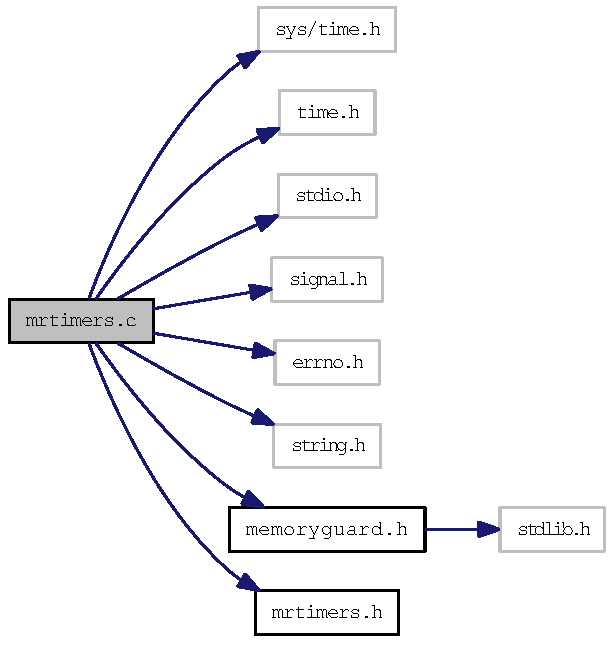
\includegraphics[width=165pt]{mrtimers_8c__incl}
\end{center}
\end{figure}
\subsection*{Data Structures}
\begin{CompactItemize}
\item 
struct \hyperlink{structTMRSysTimer}{TMRSys\-Timer}
\item 
struct \hyperlink{structTMRTimerHandler}{TMRTimer\-Handler}
\item 
struct \hyperlink{structTMRTimer}{TMRTimer}
\end{CompactItemize}
\subsection*{Defines}
\begin{CompactItemize}
\item 
\#define \hyperlink{mrtimers_8c_14497ff785c41d98a9be15617f68c063}{MRT\_\-DBG\_\-INIT\_\-MSG}~0x01
\item 
\#define \hyperlink{mrtimers_8c_632abc514382013ffc96901425623723}{MRT\_\-DBG\_\-HANDLER\_\-MSG}~0x02
\item 
\#define \hyperlink{mrtimers_8c_c5bd1b7687abdf5329151279fca0ea5b}{MRT\_\-DBG\_\-TIMER\_\-MSG}~0x04
\item 
\#define \hyperlink{mrtimers_8c_9361c4a76eaa5dc9c005e0cf2c3e4077}{MAX\_\-SYS\_\-TIMERS}~3
\item 
\#define \hyperlink{mrtimers_8c_918e72d38ef74b456fdf4be5930d6aee}{INITIAL\_\-TIMER\_\-ARRAY\_\-SIZE}~10
\end{CompactItemize}
\subsection*{Typedefs}
\begin{CompactItemize}
\item 
typedef void($\ast$) \hyperlink{mrtimers_8c_a4909967ae2a0c587ebc1b8fe7be6f9f}{sighandler\_\-t} (int)
\end{CompactItemize}
\subsection*{Functions}
\begin{CompactItemize}
\item 
int \hyperlink{mrtimers_8c_1be5b70d8f918fc6dd65a4bad657e1f3}{get\-Type\-Index\-From\-Timer\-Type} (int i\-Type)
\item 
int \hyperlink{mrtimers_8c_d14acb6d2d5840dfea0620b069869b82}{create\-Timer} (int id, int type, \hyperlink{structTMRTimer}{TMRTimer} $\ast$p\-Timer)
\item 
int \hyperlink{mrtimers_8c_9cf3aced645ad1e1ccb56d713de29748}{delete\-Timer} (int id)
\item 
\hyperlink{structTMRTimer}{TMRTimer} $\ast$ \hyperlink{mrtimers_8c_544cb64de2918fd37dfc350f240a8310}{find\-Timer\-Entry} (int $\ast$p\-ID)
\item 
void \hyperlink{mrtimers_8c_144a8348d04e0dda04351b16708de5fc}{sigalarm\-Handler} (int param)
\item 
void \hyperlink{mrtimers_8c_1b718b2ab1a0bda15118a813b608b3f7}{sigvtalarm\-Handler} (int param)
\item 
void \hyperlink{mrtimers_8c_96f4bfdf8f5792ecf27625f902384b74}{sigprof\-Handler} (int param)
\item 
int \hyperlink{mrtimers_8c_bf67f427f962506bad53c7ade379249c}{init\-MRTimers} (int i\-Base\-Time)
\item 
int \hyperlink{mrtimers_8c_7ce639af18d4674cf8e9ad36b95e76da}{release\-MRTimers} ()
\item 
int \hyperlink{mrtimers_8c_42192584a948fab8215173b75a4991b7}{set\-MRTimer\-Debug\-Flag} (int i\-Flag)
\item 
int \hyperlink{mrtimers_8c_53329aecf5a990cc91ae4355794f32ed}{clear\-MRTimer\-Debug\-Flag} (int i\-Flag)
\item 
int \hyperlink{mrtimers_8c_ccfd598b6f1a3ca5599e8bc3588d1cf7}{start\-Timer} (int i\-Type)
\item 
int \hyperlink{mrtimers_8c_bca69eeff549afdd7d72c0d011eea863}{set\-Timer\-Handler} (int id, int i\-Time\-Out\-Sec, int i\-Time\-Out\-Usec, \hyperlink{mrtimers_8h_9c199b5712594663db80db9a9ec6d6e0}{mr\-Timer\-Handler\_\-t} handler)
\item 
int \hyperlink{mrtimers_8c_fa991349587b8e300e5363a21dcee3b7}{stop\-Timer} (int id)
\item 
int \hyperlink{mrtimers_8c_60a100d9612c31984637866c7e975958}{get\-Timer\-Value} (int id, int $\ast$p\-Sec, int $\ast$p\-Usec)
\item 
const char $\ast$ \hyperlink{mrtimers_8c_eec88b57f56b75bdef646c5e44e0c2dc}{get\-Timer\-Value\-String} (int id)
\end{CompactItemize}
\subsection*{Variables}
\begin{CompactItemize}
\item 
int \hyperlink{mrtimers_8c_d49fd48232e4a34aa52e75dceb435387}{g\_\-MRTdbg\-Flags} = 0
\item 
int \hyperlink{mrtimers_8c_ea8ea38e23fffb861f535c3e4d933ced}{g\_\-systimertypes} \mbox{[}MAX\_\-SYS\_\-TIMERS\mbox{]} = \{ITIMER\_\-REAL, ITIMER\_\-VIRTUAL, ITIMER\_\-PROF\}
\item 
\hyperlink{structTMRSysTimer}{TMRSys\-Timer} \hyperlink{mrtimers_8c_a7cc6d5cbb6a544ce433ed47ae8006fd}{g\_\-systimers} \mbox{[}MAX\_\-SYS\_\-TIMERS\mbox{]}
\item 
\hyperlink{structTMRTimer}{TMRTimer} $\ast$ \hyperlink{mrtimers_8c_5b4db1e2c62e8f1bb62e4dc80bb3e378}{g\_\-array\-Timers} = NULL
\item 
int \hyperlink{mrtimers_8c_72e2c21038581ad06e38f329d8661e3c}{g\_\-array\-Timer\-Size} = 0
\item 
int \hyperlink{mrtimers_8c_251b26222e6aa201fc81e02dc657678a}{g\_\-signals} \mbox{[}MAX\_\-SYS\_\-TIMERS\mbox{]} = \{SIGALRM, SIGVTALRM, SIGPROF\}
\item 
\hyperlink{mrtimers_8c_a4909967ae2a0c587ebc1b8fe7be6f9f}{sighandler\_\-t} \hyperlink{mrtimers_8c_53abeef10d8db3cb7de4bc0b681fddc4}{g\_\-signal\-Handler} \mbox{[}MAX\_\-SYS\_\-TIMERS\mbox{]} = \{sigalarm\-Handler, sigvtalarm\-Handler, sigprof\-Handler\}
\item 
char \hyperlink{mrtimers_8c_c52e8029ebd28d6104402bc3f1f7948b}{g\_\-str\-Time} \mbox{[}20\mbox{]}
\end{CompactItemize}


\subsection{Define Documentation}
\hypertarget{mrtimers_8c_918e72d38ef74b456fdf4be5930d6aee}{
\index{mrtimers.c@{mrtimers.c}!INITIAL_TIMER_ARRAY_SIZE@{INITIAL\_\-TIMER\_\-ARRAY\_\-SIZE}}
\index{INITIAL_TIMER_ARRAY_SIZE@{INITIAL\_\-TIMER\_\-ARRAY\_\-SIZE}!mrtimers.c@{mrtimers.c}}
\subsubsection[INITIAL\_\-TIMER\_\-ARRAY\_\-SIZE]{\setlength{\rightskip}{0pt plus 5cm}\#define INITIAL\_\-TIMER\_\-ARRAY\_\-SIZE~10}}
\label{mrtimers_8c_918e72d38ef74b456fdf4be5930d6aee}




Definition at line 61 of file mrtimers.c.

Referenced by find\-Timer\-Entry().\hypertarget{mrtimers_8c_9361c4a76eaa5dc9c005e0cf2c3e4077}{
\index{mrtimers.c@{mrtimers.c}!MAX_SYS_TIMERS@{MAX\_\-SYS\_\-TIMERS}}
\index{MAX_SYS_TIMERS@{MAX\_\-SYS\_\-TIMERS}!mrtimers.c@{mrtimers.c}}
\subsubsection[MAX\_\-SYS\_\-TIMERS]{\setlength{\rightskip}{0pt plus 5cm}\#define MAX\_\-SYS\_\-TIMERS~3}}
\label{mrtimers_8c_9361c4a76eaa5dc9c005e0cf2c3e4077}




Definition at line 60 of file mrtimers.c.

Referenced by create\-Timer().\hypertarget{mrtimers_8c_632abc514382013ffc96901425623723}{
\index{mrtimers.c@{mrtimers.c}!MRT_DBG_HANDLER_MSG@{MRT\_\-DBG\_\-HANDLER\_\-MSG}}
\index{MRT_DBG_HANDLER_MSG@{MRT\_\-DBG\_\-HANDLER\_\-MSG}!mrtimers.c@{mrtimers.c}}
\subsubsection[MRT\_\-DBG\_\-HANDLER\_\-MSG]{\setlength{\rightskip}{0pt plus 5cm}\#define MRT\_\-DBG\_\-HANDLER\_\-MSG~0x02}}
\label{mrtimers_8c_632abc514382013ffc96901425623723}




Definition at line 32 of file mrtimers.c.

Referenced by sigalarm\-Handler(), sigprof\-Handler(), and sigvtalarm\-Handler().\hypertarget{mrtimers_8c_14497ff785c41d98a9be15617f68c063}{
\index{mrtimers.c@{mrtimers.c}!MRT_DBG_INIT_MSG@{MRT\_\-DBG\_\-INIT\_\-MSG}}
\index{MRT_DBG_INIT_MSG@{MRT\_\-DBG\_\-INIT\_\-MSG}!mrtimers.c@{mrtimers.c}}
\subsubsection[MRT\_\-DBG\_\-INIT\_\-MSG]{\setlength{\rightskip}{0pt plus 5cm}\#define MRT\_\-DBG\_\-INIT\_\-MSG~0x01}}
\label{mrtimers_8c_14497ff785c41d98a9be15617f68c063}




Definition at line 31 of file mrtimers.c.

Referenced by init\-MRTimers().\hypertarget{mrtimers_8c_c5bd1b7687abdf5329151279fca0ea5b}{
\index{mrtimers.c@{mrtimers.c}!MRT_DBG_TIMER_MSG@{MRT\_\-DBG\_\-TIMER\_\-MSG}}
\index{MRT_DBG_TIMER_MSG@{MRT\_\-DBG\_\-TIMER\_\-MSG}!mrtimers.c@{mrtimers.c}}
\subsubsection[MRT\_\-DBG\_\-TIMER\_\-MSG]{\setlength{\rightskip}{0pt plus 5cm}\#define MRT\_\-DBG\_\-TIMER\_\-MSG~0x04}}
\label{mrtimers_8c_c5bd1b7687abdf5329151279fca0ea5b}




Definition at line 33 of file mrtimers.c.

Referenced by create\-Timer(), delete\-Timer(), and get\-Timer\-Value().

\subsection{Typedef Documentation}
\hypertarget{mrtimers_8c_a4909967ae2a0c587ebc1b8fe7be6f9f}{
\index{mrtimers.c@{mrtimers.c}!sighandler_t@{sighandler\_\-t}}
\index{sighandler_t@{sighandler\_\-t}!mrtimers.c@{mrtimers.c}}
\subsubsection[sighandler\_\-t]{\setlength{\rightskip}{0pt plus 5cm}typedef void($\ast$) \hyperlink{mrtimers_8c_a4909967ae2a0c587ebc1b8fe7be6f9f}{sighandler\_\-t}(int)}}
\label{mrtimers_8c_a4909967ae2a0c587ebc1b8fe7be6f9f}




Definition at line 177 of file mrtimers.c.

\subsection{Function Documentation}
\hypertarget{mrtimers_8c_53329aecf5a990cc91ae4355794f32ed}{
\index{mrtimers.c@{mrtimers.c}!clearMRTimerDebugFlag@{clearMRTimerDebugFlag}}
\index{clearMRTimerDebugFlag@{clearMRTimerDebugFlag}!mrtimers.c@{mrtimers.c}}
\subsubsection[clearMRTimerDebugFlag]{\setlength{\rightskip}{0pt plus 5cm}int clear\-MRTimer\-Debug\-Flag (int {\em i\-Flag})}}
\label{mrtimers_8c_53329aecf5a990cc91ae4355794f32ed}




Definition at line 254 of file mrtimers.c.

References g\_\-MRTdbg\-Flags.

Referenced by execute\-Main\-Commands().\hypertarget{mrtimers_8c_d14acb6d2d5840dfea0620b069869b82}{
\index{mrtimers.c@{mrtimers.c}!createTimer@{createTimer}}
\index{createTimer@{createTimer}!mrtimers.c@{mrtimers.c}}
\subsubsection[createTimer]{\setlength{\rightskip}{0pt plus 5cm}int create\-Timer (int {\em id}, int {\em type}, \hyperlink{structTMRTimer}{TMRTimer} $\ast$ {\em p\-Timer})}}
\label{mrtimers_8c_d14acb6d2d5840dfea0620b069869b82}




Definition at line 81 of file mrtimers.c.

References TMRSys\-Timer::cycle\-Count, g\_\-MRTdbg\-Flags, g\_\-systimers, get\-Type\-Index\-From\-Timer\-Type(), MAX\_\-SYS\_\-TIMERS, and MRT\_\-DBG\_\-TIMER\_\-MSG.

Referenced by start\-Timer().

Here is the call graph for this function:\begin{figure}[H]
\begin{center}
\leavevmode
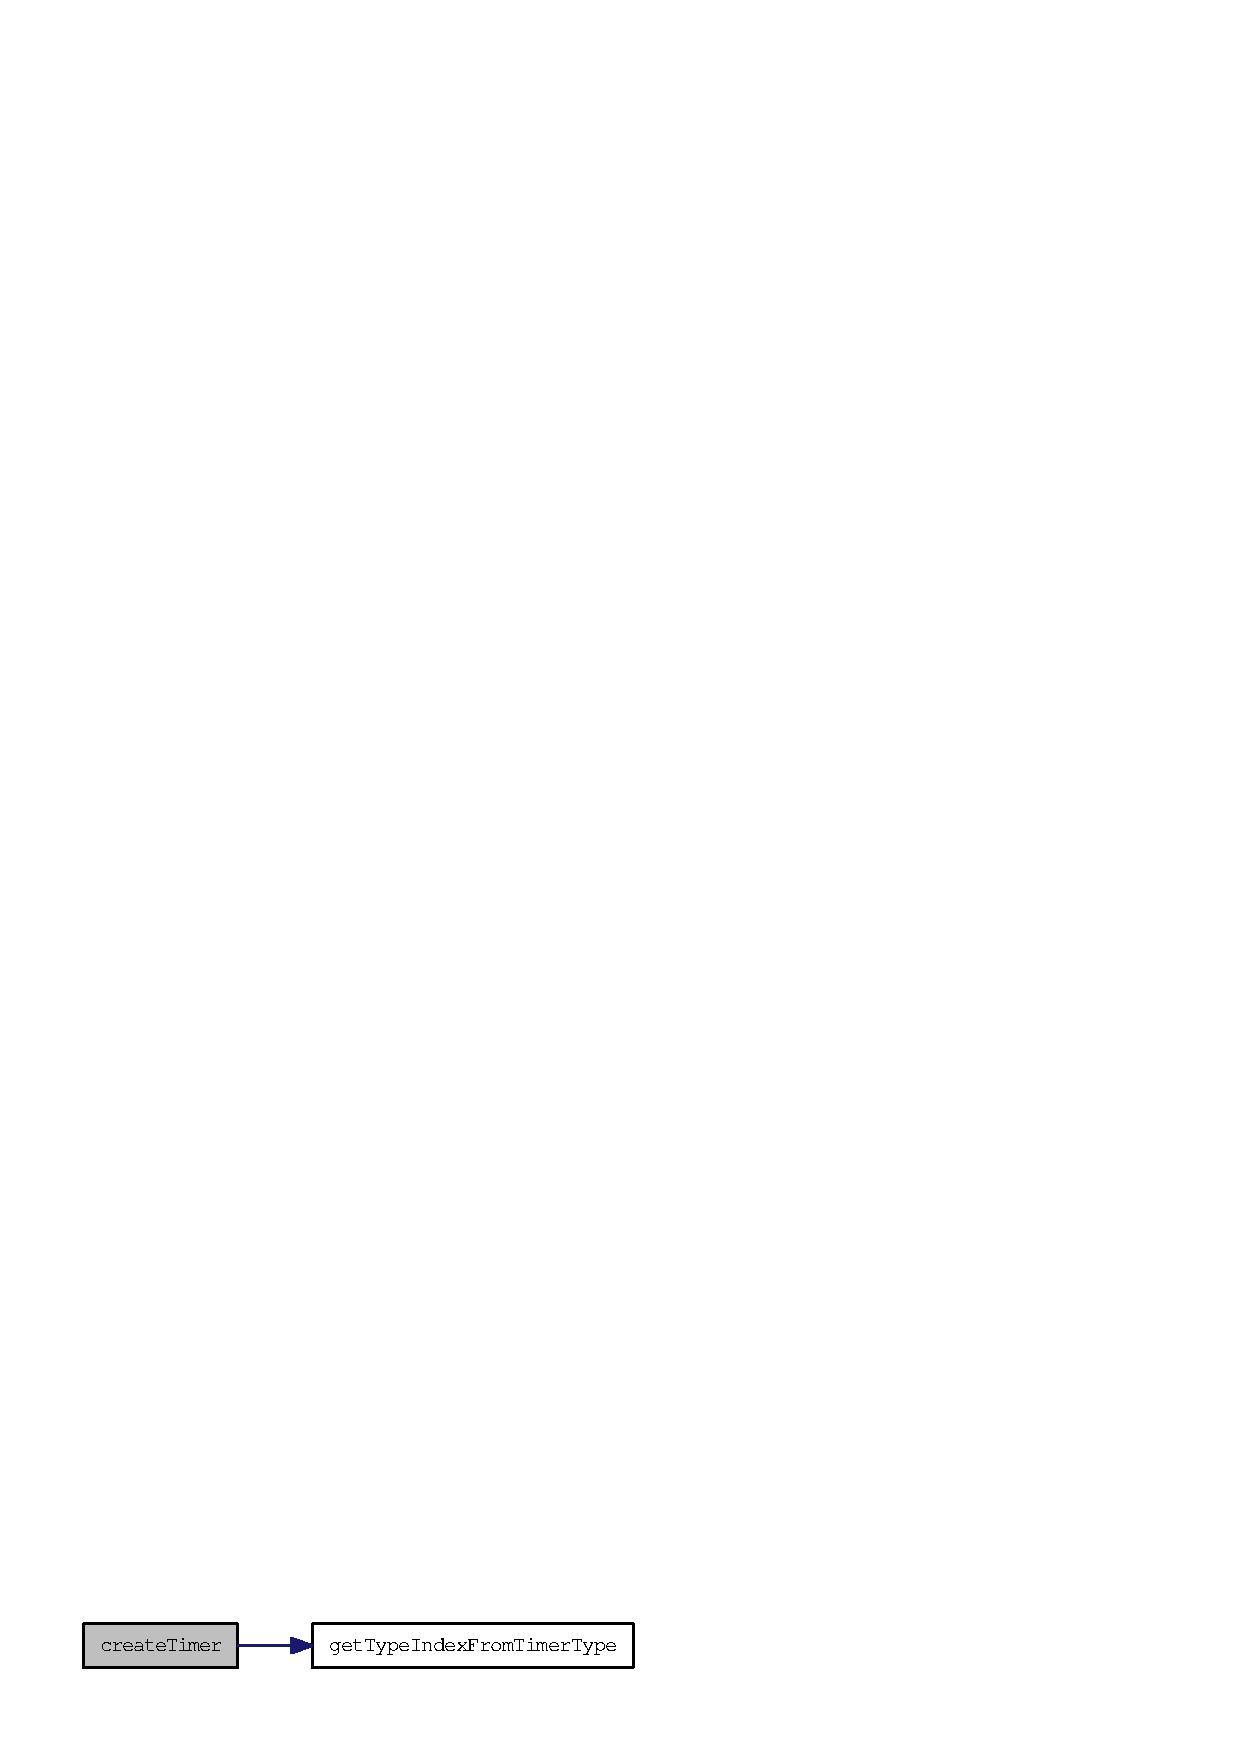
\includegraphics[width=154pt]{mrtimers_8c_d14acb6d2d5840dfea0620b069869b82_cgraph}
\end{center}
\end{figure}
\hypertarget{mrtimers_8c_9cf3aced645ad1e1ccb56d713de29748}{
\index{mrtimers.c@{mrtimers.c}!deleteTimer@{deleteTimer}}
\index{deleteTimer@{deleteTimer}!mrtimers.c@{mrtimers.c}}
\subsubsection[deleteTimer]{\setlength{\rightskip}{0pt plus 5cm}int delete\-Timer (int {\em id})}}
\label{mrtimers_8c_9cf3aced645ad1e1ccb56d713de29748}




Definition at line 104 of file mrtimers.c.

References g\_\-array\-Timers, g\_\-MRTdbg\-Flags, and MRT\_\-DBG\_\-TIMER\_\-MSG.

Referenced by stop\-Timer().\hypertarget{mrtimers_8c_544cb64de2918fd37dfc350f240a8310}{
\index{mrtimers.c@{mrtimers.c}!findTimerEntry@{findTimerEntry}}
\index{findTimerEntry@{findTimerEntry}!mrtimers.c@{mrtimers.c}}
\subsubsection[findTimerEntry]{\setlength{\rightskip}{0pt plus 5cm}\hyperlink{structTMRTimer}{TMRTimer}$\ast$ find\-Timer\-Entry (int $\ast$ {\em p\-ID})}}
\label{mrtimers_8c_544cb64de2918fd37dfc350f240a8310}




Definition at line 129 of file mrtimers.c.

References g\_\-array\-Timers, g\_\-array\-Timer\-Size, and INITIAL\_\-TIMER\_\-ARRAY\_\-SIZE.

Referenced by get\-Timer\-Value(), and start\-Timer().\hypertarget{mrtimers_8c_60a100d9612c31984637866c7e975958}{
\index{mrtimers.c@{mrtimers.c}!getTimerValue@{getTimerValue}}
\index{getTimerValue@{getTimerValue}!mrtimers.c@{mrtimers.c}}
\subsubsection[getTimerValue]{\setlength{\rightskip}{0pt plus 5cm}int get\-Timer\-Value (int {\em id}, int $\ast$ {\em p\-Sec}, int $\ast$ {\em p\-Usec})}}
\label{mrtimers_8c_60a100d9612c31984637866c7e975958}




Definition at line 285 of file mrtimers.c.

References TMRSys\-Timer::cycle\-Count, find\-Timer\-Entry(), g\_\-MRTdbg\-Flags, g\_\-systimers, MRT\_\-DBG\_\-TIMER\_\-MSG, TMRTimer::startcycle, TMRTimer::startvalue, and TMRTimer::type\-Index.

Referenced by get\-Timer\-Value\-String(), timed\-Wait(), and wait\-Condition().

Here is the call graph for this function:\begin{figure}[H]
\begin{center}
\leavevmode
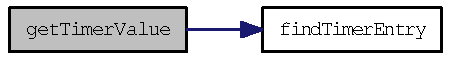
\includegraphics[width=126pt]{mrtimers_8c_60a100d9612c31984637866c7e975958_cgraph}
\end{center}
\end{figure}
\hypertarget{mrtimers_8c_eec88b57f56b75bdef646c5e44e0c2dc}{
\index{mrtimers.c@{mrtimers.c}!getTimerValueString@{getTimerValueString}}
\index{getTimerValueString@{getTimerValueString}!mrtimers.c@{mrtimers.c}}
\subsubsection[getTimerValueString]{\setlength{\rightskip}{0pt plus 5cm}const char$\ast$ get\-Timer\-Value\-String (int {\em id})}}
\label{mrtimers_8c_eec88b57f56b75bdef646c5e44e0c2dc}




Definition at line 323 of file mrtimers.c.

References g\_\-str\-Time, and get\-Timer\-Value().

Referenced by exec\-Batch(), and exec\-Write\-Cmd().

Here is the call graph for this function:\begin{figure}[H]
\begin{center}
\leavevmode
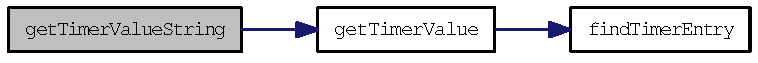
\includegraphics[width=200pt]{mrtimers_8c_eec88b57f56b75bdef646c5e44e0c2dc_cgraph}
\end{center}
\end{figure}
\hypertarget{mrtimers_8c_1be5b70d8f918fc6dd65a4bad657e1f3}{
\index{mrtimers.c@{mrtimers.c}!getTypeIndexFromTimerType@{getTypeIndexFromTimerType}}
\index{getTypeIndexFromTimerType@{getTypeIndexFromTimerType}!mrtimers.c@{mrtimers.c}}
\subsubsection[getTypeIndexFromTimerType]{\setlength{\rightskip}{0pt plus 5cm}int get\-Type\-Index\-From\-Timer\-Type (int {\em i\-Type})}}
\label{mrtimers_8c_1be5b70d8f918fc6dd65a4bad657e1f3}




Definition at line 67 of file mrtimers.c.

Referenced by create\-Timer().\hypertarget{mrtimers_8c_bf67f427f962506bad53c7ade379249c}{
\index{mrtimers.c@{mrtimers.c}!initMRTimers@{initMRTimers}}
\index{initMRTimers@{initMRTimers}!mrtimers.c@{mrtimers.c}}
\subsubsection[initMRTimers]{\setlength{\rightskip}{0pt plus 5cm}int init\-MRTimers (int {\em i\-Base\-Time})}}
\label{mrtimers_8c_bf67f427f962506bad53c7ade379249c}




Definition at line 184 of file mrtimers.c.

References TMRSys\-Timer::cycle\-Count, g\_\-array\-Timers, g\_\-array\-Timer\-Size, g\_\-MRTdbg\-Flags, g\_\-signal\-Handler, g\_\-signals, g\_\-systimers, g\_\-systimertypes, and MRT\_\-DBG\_\-INIT\_\-MSG.

Referenced by main().\hypertarget{mrtimers_8c_7ce639af18d4674cf8e9ad36b95e76da}{
\index{mrtimers.c@{mrtimers.c}!releaseMRTimers@{releaseMRTimers}}
\index{releaseMRTimers@{releaseMRTimers}!mrtimers.c@{mrtimers.c}}
\subsubsection[releaseMRTimers]{\setlength{\rightskip}{0pt plus 5cm}int release\-MRTimers ()}}
\label{mrtimers_8c_7ce639af18d4674cf8e9ad36b95e76da}




Definition at line 236 of file mrtimers.c.

References g\_\-array\-Timers, and g\_\-array\-Timer\-Size.

Referenced by main().\hypertarget{mrtimers_8c_42192584a948fab8215173b75a4991b7}{
\index{mrtimers.c@{mrtimers.c}!setMRTimerDebugFlag@{setMRTimerDebugFlag}}
\index{setMRTimerDebugFlag@{setMRTimerDebugFlag}!mrtimers.c@{mrtimers.c}}
\subsubsection[setMRTimerDebugFlag]{\setlength{\rightskip}{0pt plus 5cm}int set\-MRTimer\-Debug\-Flag (int {\em i\-Flag})}}
\label{mrtimers_8c_42192584a948fab8215173b75a4991b7}




Definition at line 248 of file mrtimers.c.

References g\_\-MRTdbg\-Flags.

Referenced by execute\-Main\-Commands().\hypertarget{mrtimers_8c_bca69eeff549afdd7d72c0d011eea863}{
\index{mrtimers.c@{mrtimers.c}!setTimerHandler@{setTimerHandler}}
\index{setTimerHandler@{setTimerHandler}!mrtimers.c@{mrtimers.c}}
\subsubsection[setTimerHandler]{\setlength{\rightskip}{0pt plus 5cm}int set\-Timer\-Handler (int {\em id}, int {\em i\-Time\-Out\-Sec}, int {\em i\-Time\-Out\-Usec}, \hyperlink{mrtimers_8h_9c199b5712594663db80db9a9ec6d6e0}{mr\-Timer\-Handler\_\-t} {\em handler})}}
\label{mrtimers_8c_bca69eeff549afdd7d72c0d011eea863}




Definition at line 273 of file mrtimers.c.\hypertarget{mrtimers_8c_144a8348d04e0dda04351b16708de5fc}{
\index{mrtimers.c@{mrtimers.c}!sigalarmHandler@{sigalarmHandler}}
\index{sigalarmHandler@{sigalarmHandler}!mrtimers.c@{mrtimers.c}}
\subsubsection[sigalarmHandler]{\setlength{\rightskip}{0pt plus 5cm}void sigalarm\-Handler (int {\em param})}}
\label{mrtimers_8c_144a8348d04e0dda04351b16708de5fc}




Definition at line 159 of file mrtimers.c.

References TMRSys\-Timer::cycle\-Count, g\_\-MRTdbg\-Flags, g\_\-systimers, and MRT\_\-DBG\_\-HANDLER\_\-MSG.\hypertarget{mrtimers_8c_96f4bfdf8f5792ecf27625f902384b74}{
\index{mrtimers.c@{mrtimers.c}!sigprofHandler@{sigprofHandler}}
\index{sigprofHandler@{sigprofHandler}!mrtimers.c@{mrtimers.c}}
\subsubsection[sigprofHandler]{\setlength{\rightskip}{0pt plus 5cm}void sigprof\-Handler (int {\em param})}}
\label{mrtimers_8c_96f4bfdf8f5792ecf27625f902384b74}




Definition at line 171 of file mrtimers.c.

References TMRSys\-Timer::cycle\-Count, g\_\-MRTdbg\-Flags, g\_\-systimers, and MRT\_\-DBG\_\-HANDLER\_\-MSG.\hypertarget{mrtimers_8c_1b718b2ab1a0bda15118a813b608b3f7}{
\index{mrtimers.c@{mrtimers.c}!sigvtalarmHandler@{sigvtalarmHandler}}
\index{sigvtalarmHandler@{sigvtalarmHandler}!mrtimers.c@{mrtimers.c}}
\subsubsection[sigvtalarmHandler]{\setlength{\rightskip}{0pt plus 5cm}void sigvtalarm\-Handler (int {\em param})}}
\label{mrtimers_8c_1b718b2ab1a0bda15118a813b608b3f7}




Definition at line 165 of file mrtimers.c.

References TMRSys\-Timer::cycle\-Count, g\_\-MRTdbg\-Flags, g\_\-systimers, and MRT\_\-DBG\_\-HANDLER\_\-MSG.\hypertarget{mrtimers_8c_ccfd598b6f1a3ca5599e8bc3588d1cf7}{
\index{mrtimers.c@{mrtimers.c}!startTimer@{startTimer}}
\index{startTimer@{startTimer}!mrtimers.c@{mrtimers.c}}
\subsubsection[startTimer]{\setlength{\rightskip}{0pt plus 5cm}int start\-Timer (int {\em i\-Type})}}
\label{mrtimers_8c_ccfd598b6f1a3ca5599e8bc3588d1cf7}




Definition at line 260 of file mrtimers.c.

References create\-Timer(), and find\-Timer\-Entry().

Referenced by exec\-Batch(), exec\-Write\-Cmd(), timed\-Wait(), and wait\-Condition().

Here is the call graph for this function:\begin{figure}[H]
\begin{center}
\leavevmode
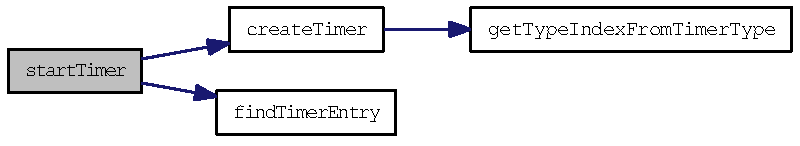
\includegraphics[width=210pt]{mrtimers_8c_ccfd598b6f1a3ca5599e8bc3588d1cf7_cgraph}
\end{center}
\end{figure}
\hypertarget{mrtimers_8c_fa991349587b8e300e5363a21dcee3b7}{
\index{mrtimers.c@{mrtimers.c}!stopTimer@{stopTimer}}
\index{stopTimer@{stopTimer}!mrtimers.c@{mrtimers.c}}
\subsubsection[stopTimer]{\setlength{\rightskip}{0pt plus 5cm}int stop\-Timer (int {\em id})}}
\label{mrtimers_8c_fa991349587b8e300e5363a21dcee3b7}




Definition at line 279 of file mrtimers.c.

References delete\-Timer().

Referenced by exec\-Batch(), exec\-Write\-Cmd(), timed\-Wait(), and wait\-Condition().

Here is the call graph for this function:\begin{figure}[H]
\begin{center}
\leavevmode
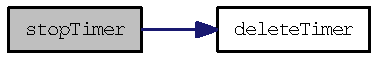
\includegraphics[width=109pt]{mrtimers_8c_fa991349587b8e300e5363a21dcee3b7_cgraph}
\end{center}
\end{figure}


\subsection{Variable Documentation}
\hypertarget{mrtimers_8c_5b4db1e2c62e8f1bb62e4dc80bb3e378}{
\index{mrtimers.c@{mrtimers.c}!g_arrayTimers@{g\_\-arrayTimers}}
\index{g_arrayTimers@{g\_\-arrayTimers}!mrtimers.c@{mrtimers.c}}
\subsubsection[g\_\-arrayTimers]{\setlength{\rightskip}{0pt plus 5cm}\hyperlink{structTMRTimer}{TMRTimer}$\ast$ \hyperlink{mrtimers_8c_5b4db1e2c62e8f1bb62e4dc80bb3e378}{g\_\-array\-Timers} = NULL}}
\label{mrtimers_8c_5b4db1e2c62e8f1bb62e4dc80bb3e378}




Definition at line 64 of file mrtimers.c.

Referenced by delete\-Timer(), find\-Timer\-Entry(), init\-MRTimers(), and release\-MRTimers().\hypertarget{mrtimers_8c_72e2c21038581ad06e38f329d8661e3c}{
\index{mrtimers.c@{mrtimers.c}!g_arrayTimerSize@{g\_\-arrayTimerSize}}
\index{g_arrayTimerSize@{g\_\-arrayTimerSize}!mrtimers.c@{mrtimers.c}}
\subsubsection[g\_\-arrayTimerSize]{\setlength{\rightskip}{0pt plus 5cm}int \hyperlink{mrtimers_8c_72e2c21038581ad06e38f329d8661e3c}{g\_\-array\-Timer\-Size} = 0}}
\label{mrtimers_8c_72e2c21038581ad06e38f329d8661e3c}




Definition at line 65 of file mrtimers.c.

Referenced by find\-Timer\-Entry(), init\-MRTimers(), and release\-MRTimers().\hypertarget{mrtimers_8c_d49fd48232e4a34aa52e75dceb435387}{
\index{mrtimers.c@{mrtimers.c}!g_MRTdbgFlags@{g\_\-MRTdbgFlags}}
\index{g_MRTdbgFlags@{g\_\-MRTdbgFlags}!mrtimers.c@{mrtimers.c}}
\subsubsection[g\_\-MRTdbgFlags]{\setlength{\rightskip}{0pt plus 5cm}int \hyperlink{mrtimers_8c_d49fd48232e4a34aa52e75dceb435387}{g\_\-MRTdbg\-Flags} = 0}}
\label{mrtimers_8c_d49fd48232e4a34aa52e75dceb435387}




Definition at line 34 of file mrtimers.c.

Referenced by clear\-MRTimer\-Debug\-Flag(), create\-Timer(), delete\-Timer(), get\-Timer\-Value(), init\-MRTimers(), set\-MRTimer\-Debug\-Flag(), sigalarm\-Handler(), sigprof\-Handler(), and sigvtalarm\-Handler().\hypertarget{mrtimers_8c_53abeef10d8db3cb7de4bc0b681fddc4}{
\index{mrtimers.c@{mrtimers.c}!g_signalHandler@{g\_\-signalHandler}}
\index{g_signalHandler@{g\_\-signalHandler}!mrtimers.c@{mrtimers.c}}
\subsubsection[g\_\-signalHandler]{\setlength{\rightskip}{0pt plus 5cm}\hyperlink{mrtimers_8c_a4909967ae2a0c587ebc1b8fe7be6f9f}{sighandler\_\-t} \hyperlink{mrtimers_8c_53abeef10d8db3cb7de4bc0b681fddc4}{g\_\-signal\-Handler}\mbox{[}MAX\_\-SYS\_\-TIMERS\mbox{]} = \{sigalarm\-Handler, sigvtalarm\-Handler, sigprof\-Handler\}}}
\label{mrtimers_8c_53abeef10d8db3cb7de4bc0b681fddc4}




Definition at line 179 of file mrtimers.c.

Referenced by init\-MRTimers().\hypertarget{mrtimers_8c_251b26222e6aa201fc81e02dc657678a}{
\index{mrtimers.c@{mrtimers.c}!g_signals@{g\_\-signals}}
\index{g_signals@{g\_\-signals}!mrtimers.c@{mrtimers.c}}
\subsubsection[g\_\-signals]{\setlength{\rightskip}{0pt plus 5cm}int \hyperlink{mrtimers_8c_251b26222e6aa201fc81e02dc657678a}{g\_\-signals}\mbox{[}MAX\_\-SYS\_\-TIMERS\mbox{]} = \{SIGALRM, SIGVTALRM, SIGPROF\}}}
\label{mrtimers_8c_251b26222e6aa201fc81e02dc657678a}




Definition at line 178 of file mrtimers.c.

Referenced by init\-MRTimers().\hypertarget{mrtimers_8c_c52e8029ebd28d6104402bc3f1f7948b}{
\index{mrtimers.c@{mrtimers.c}!g_strTime@{g\_\-strTime}}
\index{g_strTime@{g\_\-strTime}!mrtimers.c@{mrtimers.c}}
\subsubsection[g\_\-strTime]{\setlength{\rightskip}{0pt plus 5cm}char \hyperlink{mrtimers_8c_c52e8029ebd28d6104402bc3f1f7948b}{g\_\-str\-Time}\mbox{[}20\mbox{]}}}
\label{mrtimers_8c_c52e8029ebd28d6104402bc3f1f7948b}




Definition at line 322 of file mrtimers.c.

Referenced by get\-Timer\-Value\-String().\hypertarget{mrtimers_8c_a7cc6d5cbb6a544ce433ed47ae8006fd}{
\index{mrtimers.c@{mrtimers.c}!g_systimers@{g\_\-systimers}}
\index{g_systimers@{g\_\-systimers}!mrtimers.c@{mrtimers.c}}
\subsubsection[g\_\-systimers]{\setlength{\rightskip}{0pt plus 5cm}\hyperlink{structTMRSysTimer}{TMRSys\-Timer} \hyperlink{mrtimers_8c_a7cc6d5cbb6a544ce433ed47ae8006fd}{g\_\-systimers}\mbox{[}MAX\_\-SYS\_\-TIMERS\mbox{]}}}
\label{mrtimers_8c_a7cc6d5cbb6a544ce433ed47ae8006fd}




Definition at line 63 of file mrtimers.c.

Referenced by create\-Timer(), get\-Timer\-Value(), init\-MRTimers(), sigalarm\-Handler(), sigprof\-Handler(), and sigvtalarm\-Handler().\hypertarget{mrtimers_8c_ea8ea38e23fffb861f535c3e4d933ced}{
\index{mrtimers.c@{mrtimers.c}!g_systimertypes@{g\_\-systimertypes}}
\index{g_systimertypes@{g\_\-systimertypes}!mrtimers.c@{mrtimers.c}}
\subsubsection[g\_\-systimertypes]{\setlength{\rightskip}{0pt plus 5cm}int \hyperlink{mrtimers_8c_ea8ea38e23fffb861f535c3e4d933ced}{g\_\-systimertypes}\mbox{[}MAX\_\-SYS\_\-TIMERS\mbox{]} = \{ITIMER\_\-REAL, ITIMER\_\-VIRTUAL, ITIMER\_\-PROF\}}}
\label{mrtimers_8c_ea8ea38e23fffb861f535c3e4d933ced}




Definition at line 62 of file mrtimers.c.

Referenced by init\-MRTimers().